\documentclass[twoside]{article}
\input{ISC18-english.sty}
%%%%%%%%%%%%%%%%%%%%%%%%%%%%  Make sure to compile twice for proper cross-references. %%%%%%%%%%%%%%%%%%%%%%%
%%%%%%% For proper display of references, compile the document twice. %%%%%%%%%%%%%%%%%%%%% 
%%%%%%%%%%%%%%% If using TeX Live, compile using pdflatex command %%%%%%%%%%%%%%%%%%%%%%%
\usepackage{xfrac}
\begin{document}
\thispagestyle{empty}
%%%%%%%%%%%%%%%%% Article title header  %%%%%%%%%%%%%%%%%%%%
\fancyhead[LE]{Bayesian Learning of Gene Expression Networks}
%%%%%%%%%%%%%%%%% Article authors header   %%%%%%%%%%%%%%%%%%%%
\fancyhead[RO]{Nazari et al.}
\vspace*{-3cm}
\begin{center}
{
\includegraphics [height=25mm, width=150.3mm] {Images/isc18E}} \\
%\vspace*{-1.8cm}
%\begin{center}
%\color{blue} 
%{\hspace{0.1cm}\rule{\textwidth}{1mm}}\\
%\end{center}
\vspace*{1cm}
%%%%%%%%%%%%%%%%% Article title  %%%%%%%%%%%%%%%%%%%%
{\Large \bf Bayesian Structure Learning of Gene Expression Networks via Laplace-Approximated Scoring: An Application to TCGA Breast Cancer Data}\\
%%%%%%%%%%%%%%%%% Article authors and affiliations %%%%%%%%%%%%%%%%%%%%
{\bf
Samaneh Nazari\textsuperscript{1,*}, Mohammad Arashi\textsuperscript{1}, and Abdolnasser Sadeghkhani\textsuperscript{2} \\
\begingroup
\renewcommand{\thefootnote}{}
\footnotetext{\textsuperscript{*}Corresponding author, \texttt{email: asemaneh1369@gmail.com}}
\endgroup
$^1$Department of Statistics, Faculty of Mathematical Sciences, Ferdowsi University of Mashhad, P. O. Box 1159, Mashhad 91775, Iran \\
$^2$Department of Mathematics and Statistics, North Carolina Agricultural and Technical State University, USA}
\end{center}
\vspace{-1cm}
\rule{\textwidth}{0.2mm}\\
%%%%%%%%%%%%%%%%% Article abstract  %%%%%%%%%%%%%%%%%%%%
\noindent{\bf Abstract:}\\
Breast cancer is a heterogeneous disease driven by complex molecular interactions. 
Identifying direct dependencies between continuous gene expression profiles and discrete clinical outcomes is critical to robust biomarker discovery. 
In this study, we present an empirical application of a recently developed Bayesian directed acyclic graph (DAG) learning framework to infer probabilistic dependency networks from the TCGA Breast Cancer dataset. 
The proposed framework utilizes a DAG-Probit model, treating the binary clinical status as a thresholded latent Gaussian variable.
By leveraging Laplace approximations to efficiently estimate node-wise marginal likelihoods and employing Markov chain Monte Carlo (MCMC) sampling for high-dimensional structure exploration, the model successfully infers a sparse, clinically relevant regulatory network. 
The application identifies key driver genes—such as \textit{COL11A1}, \textit{PCOLCE2}, and \textit{SFRP1}—with a posterior edge inclusion probability ($1.00$), demonstrating the effectiveness of the framework for biological interpretation and mechanistic oncology studies.
 
\noindent{\bf Keywords:} 
Bayesian Structure Learning, Breast Cancer Data, DAG-Probit Model, Gene Regulatory Networks, Mixed Data. \\
\noindent{\bf Mathematics Subject Classification (2010):} $\rm 62P10$, $\rm 62F15$, $\rm 62H22
$. \\
\hspace{1cm}\rule{\textwidth}{0.2mm}
%%%%%%%%%%%%%%
\section{Introduction}
\label{sec:introduction}

Understanding the intricate regulatory mechanisms underlying complex diseases, such as breast cancer, is a primary objective in modern genomics \citep{CGAN12}.
Gene regulatory networks (GRNs) modeled by directed acyclic graphs (DAGs) have emerged as powerful tools to decipher these interactions, offering probabilistic representations of causal dependencies between genetic biomarkers \citep{Friedman00}.
However, a significant methodological challenge arises when attempting to integrate high-dimensional continuous transcriptomic data with discrete clinical outcomes within a unified structural learning framework.

To address this challenge, a Bayesian directed acyclic graph structure learning framework for DAG-probit models provides a robust mathematical solution \citep{Castelletti21}. 
This approach utilizes a latent probit model to bridge the gap between binary clinical variables and continuous gene expression data. 
Specifically, our study adopts a recently developed Bayesian framework tailored for the structure learning of DAG-probit models \citep{Nazari:2026}. 
This methodology introduces a novel prior distribution and uses a Laplace approximation to efficiently compute the Bayesian scoring metric required for accurate and scalable structure learning.

Building upon the theoretical foundations of this framework, the present study investigates its practical utility and biological relevance. 
Our primary contribution lies in the empirical validation of this methodology using real-world clinical data. 
By applying the DAG-probit approach to the TCGA breast cancer dataset--comprising the top 50 differentially expressed genes alongside binary tissue status--we reconstruct the underlying gene regulatory network. 
This application enables the quantification of structural uncertainties and the explicit identification of key regulatory interactions associated with the disease state.

The remainder of this paper is organized as follows. Section \ref{sec:methodology} details the methodology, followed by data description and preprocessing in Section \ref{sec:data}; Section \ref{sec:application} presents the application results, and concluding remarks are provided in the final section.
\vspace{-1.4cm}\section{Methodology}
\label{sec:methodology}

This study adopts the Bayesian framework proposed by \cite{Nazari:2026} for structural learning in gene regulatory networks. 
Given a data set of continuous features (e.g., gene expressions) and a binary response (e.g., clinical outcome), we model the dependencies using a DAG and incorporate the binary outcome as a latent variable thresholded by a probit link.

\subsection{Network Model and Modified Cholesky Parameterization}
\label{subsec:MChD}

Let $\mathcal{D} = (V, E)$ denote a DAG comprising $q$ nodes. We assume a reverse-topological ordering of the nodes, in which node $1$ designates the latent outcome variable, constraining it as a terminal node without children. Assuming that the random vector $\boldsymbol{X} = (X_1, \ldots, X_q)^T$ follows a zero-mean multivariate Gaussian distribution, $\boldsymbol{X} \sim \mathcal{N}_q(\boldsymbol{0}, \boldsymbol{\Omega}^{-1})$, which satisfies the Markov property with respect to $\mathcal{D}$, we impose the structural constraints of the DAG by parameterizing the precision matrix $\boldsymbol{\Omega}$ via the modified Cholesky decomposition, $\boldsymbol{\Omega} = \boldsymbol{L} \boldsymbol{D}^{-1} \boldsymbol{L}^T$. In this formulation, $\boldsymbol{L}$ is a unit lower triangular matrix and $\boldsymbol{D} = \text{diag}(\sigma_{1}^{2}, \ldots, \sigma_{q}^{2})$ represents a diagonal matrix of residual variances.

This parameterization permits an interpretation of the structural equation model, where the $j$-th node can be expressed as a linear regression of its parents in the DAG:
\begin{equation*}
	X_j = - \boldsymbol{L}_{\prec j \rbrack}^T \boldsymbol{X}_{pa_D(j)} + \varepsilon_j, \quad \varepsilon_j \mid \sigma_j^2 \overset{iid}{\sim} \mathcal{N}(0, \sigma_j^2)	
\end{equation*}
Here, the model enforces $L_{u,j} \neq 0$ if and only if $u \in pa_D(j)$, thereby directly mapping the structural constraints of the graph in the regression coefficients. 
Additionally, $\boldsymbol{L}_{\prec j]}$ denotes the $j$-th column of $\boldsymbol{L}$ restricted to the rows indexed by the parent set, $pa_{\mathcal{D}}(j)$.

To incorporate the binary clinical status $Y\in\lbrace0,1\rbrace$ (normal vs. tumor) into the DAG framework, we represent $Y$ as a thresholded realization of a latent Gaussian variable $X_1$, such that
 $Y = \mathbb{I}(X_1 \geq \theta_0)$.
To ensure the identifiability of the model, the variance of this latent variable is fixed at $\sigma_1^2 = 1$. 
Furthermore, by enforcing a specific topological ordering, $X_{1}$ is restricted to being a sink node, which guaranties that the model captures the directional effects from genes to clinical status without allowing biologically implausible reverse causality.

\vspace{-0.3cm}\subsection{Prior Elicitation}
We employ a non-conjugate Normal-Gamma prior to regularizing both the DAG structure and its parameters. For the DAG topology, let $\boldsymbol{A}^{\mathcal{D}}$ be the symmetric $0-1$ adjacency matrix corresponding to the skeleton of $\mathcal{D}$, whose $(u, v)$-element is denoted by $A^{\mathcal{D}}_{u,v}$. We assign a Bernoulli prior independently to each element in the lower-triangular part of $\boldsymbol{A}^{\mathcal{D}}$, that is, $A^{\mathcal{D}}_{u,v} \stackrel{iid}{\sim} \text{Ber}(\pi)$ for $u > v$. This implies that each edge exists independently with probability $\pi \in [0,1]$, yielding the following prior on the DAG $\mathcal{D}$:
\begin{equation*}
	p(\mathcal{D}) \propto \pi^{\lvert\boldsymbol{A}^{\mathcal{D}}\rvert} (1-\pi)^{\sfrac{q(q-1)}{2} - \lvert\boldsymbol{A}^{\mathcal{D}}\rvert},
\end{equation*}
where $\lvert\boldsymbol{A}^{\mathcal{D}}\rvert = \sum_{u>v} A^{\mathcal{D}}_{u,v}$ denotes the total number of edges in the skeleton.

Conditioned on the graph structure, the parameters of the continuous nodes ($j \in \{2, \dots, q\}$) are assigned a Normal-Gamma specification:
\begin{equation*}
	\sigma_j^2 \mid \mathcal{D} \sim \text{Gamma}\left( \frac{1}{2} \alpha_{j}^{\mathcal{D}}, \frac{g}{2} \right), \quad \boldsymbol{L}_{\prec j \rbrack} \mid \sigma_j^2, \mathcal{D} \sim \mathcal{N}_{\lvert \text{pa}_{\mathcal{D}}(j)\rvert}\left(\boldsymbol{0}, \frac{\sigma_{j}^{2}}{g} \boldsymbol{I}_{\lvert \text{pa}_{\mathcal{D}}(j)\rvert}\right),
\end{equation*}
where $g$ is a hyperparameter (set to $g=2$), and $\alpha_{j}^{\mathcal{D}}$ is a function of the degree of the node designed to ensure the consistency of the model and appropriate shrinkage. For the response node ($j=1$), to ensure the identifiability of the probit model, the variance is fixed at $\sigma_1^2 = 1$.
%, yielding a marginal Normal prior for its parent coefficients: 
%\begin{equation*}
 %   \boldsymbol{L}_{\prec 1 \rbrack} \mid \mathcal{D} \sim \mathcal{N}_{\lvert \text{pa}_{\mathcal{D}}(1)\rvert}\left(\boldsymbol{0}, \frac{1}{g} \boldsymbol{I}_{\lvert \text{pa}_{\mathcal{D}}(1)\rvert}\right).
%\end{equation*}
Finally, we assign an improper uniform prior for the threshold parameter, $p(\theta_0) \propto 1$.

\vspace{-0.3cm}\subsection{Bayesian Scoring and Posterior Inference}
For the continuous nodes ($j \in \{2, \ldots, q\}$), the non-conjugacy of the Normal-Gamma prior means that the marginal likelihood lacks a closed form. We adopt the Laplace-approximated Bayesian scoring function defined in \cite{Nazari:2026}. Given an $n \times q$ observation matrix $\boldsymbol{X}$, we define $\boldsymbol{M}_j = \boldsymbol{X}_{\text{pa}_{\mathcal{D}}(j)}^{T}\boldsymbol{X}_{\text{pa}_{\mathcal{D}}(j)} + g\,\boldsymbol{I}_{\lvert \text{pa}_{\mathcal{D}}(j)\rvert}$, $\boldsymbol{b}_j = -\boldsymbol{X}_{\text{pa}_{\mathcal{D}}(j)}^{T}\boldsymbol{X}_j$, and $\kappa_j = \frac{1}{2}( -\boldsymbol{b}_j^{T}\boldsymbol{M}_j^{-1}\boldsymbol{b}_j + \boldsymbol{X}_j^{T}\boldsymbol{X}_j )$. With $\lambda = \frac{1}{2}g$ and $a = \frac{1}{2}\alpha_j^{\mathcal{D}} - \frac{n}{2}$, the Laplace-approximated node-marginal likelihood is:
\begin{equation*}
	\hat{l}(\boldsymbol{X}_j \mid \boldsymbol{X}_{\text{pa}_{\mathcal{D}}(j)}, \mathcal{D}) \propto \lvert\boldsymbol{M}_j^{-1}\rvert^{1/2} \left(\dfrac{\kappa_j^{2a-1}}{\lambda^{2a+1}}\right)^{1/4}\exp\left(-2\sqrt{\kappa_j \lambda}\right).
\end{equation*}

Conditional on the DAG, the corresponding posterior distributions are $\boldsymbol{L}_{\prec j\rbrack} \mid \sigma_j^2, \mathcal{D}, \boldsymbol{X} \sim \mathcal{N} (\boldsymbol{M}_j^{-1}\boldsymbol{b}_j, \sigma_j^2 \boldsymbol{M}_j^{-1})$ and 
$\sigma_j^2 \mid \mathcal{D}, \boldsymbol{X} \sim \text{GIG}\left(a, 2\lambda, 2\kappa_j\right)$, where \text{GIG} denotes the Generalized Inverse Gaussian distribution.

In contrast, for the latent variable of the binary clinical outcome ($j = 1$), the identifiability constraint $\sigma_1^2 = 1$ leads to a conjugate formulation. Defining $\boldsymbol{S}_1 = g\boldsymbol{I}_{\lvert\text{pa}_{\mathcal{D}}(1)\rvert}$, $\boldsymbol{M}_1 = \boldsymbol{S}_1 + \boldsymbol{X}_{\text{pa}_{\mathcal{D}}(1)}^{T}\boldsymbol{X}_{\text{pa}_{\mathcal{D}}(1)}$, and $\boldsymbol{\gamma}_1 = \boldsymbol{M}_1^{-1}\boldsymbol{X}_{\text{pa}_{\mathcal{D}}(1)}^{T}\boldsymbol{X}_1$, the exact marginal likelihood is given by:
\begin{equation*}
	l(\boldsymbol{X}_1 \mid \boldsymbol{X}_{\text{pa}_{\mathcal{D}}(1)}, \mathcal{D}) = (2\pi)^{-\frac{n}{2}} \frac{\lvert\boldsymbol{S}_1\rvert^{\frac{1}{2}}}{\lvert\boldsymbol{M}_1\rvert^{\frac{1}{2}}} \exp\left\{-\frac{1}{2}\left(\boldsymbol{X}_1^{T}\boldsymbol{X}_1 - \boldsymbol{\gamma}_1^{T}\boldsymbol{M}_1\boldsymbol{\gamma}_1\right)\right\}.
\end{equation*}
The exact posterior distribution of its parameters is simply $\boldsymbol{L}_{\prec 1\rbrack} \mid \boldsymbol{X} \sim \mathcal{N}_{\lvert\text{pa}_{\mathcal{D}}(1)\rvert} (-\boldsymbol{\gamma}_1, \boldsymbol{M}_1^{-1})$.

\vspace{-0.3cm}\subsection{Structure Search and MCMC Inference}
To explore the posterior distribution of DAGs, we employed a Metropolis–Hastings Markov Chain Monte Carlo (MCMC) algorithm. The sampler makes moves in the space of DAGs—specifically $\text{Insert}(i \to j)$, $\text{Delete}(i \to j)$, and $\text{Reverse}(i \to j)$—to update the graph structure, subject to the acyclicity constraint. Within each iteration, we employ Gibbs steps to update the continuous parameters $\left(\boldsymbol{L},\boldsymbol{D}\right)$ and the latent observations $X_1$, while the threshold $\theta_0$ is updated by a random-walk Metropolis step, ensuring comprehensive sampling of the posterior space.

\section{Data Description and Preprocessing}
\label{sec:data}
\vspace{-0.3cm}
The proposed methodology is evaluated on a breast cancer gene expression dataset sourced from The Cancer Genome Atlas (TCGA). The dataset comprises Log2-normalized RNA-sequencing profiles from  patient samples $n=590$. Each sample is associated with a binary clinical diagnosis, categorizing the tissue as Normal ($61$ samples) or Tumor ($529$ samples). Initially, the raw dataset includes $17,814$ gene expression features per sample, which presents a high-dimensional challenge typical in cancer genomics.

\vspace{-0.7cm}\subsection{Data Preprocessing}
To prepare the transcriptomic data for the Bayesian structure learning framework, a systematic preprocessing pipeline was applied. First, the independent Normal and Tumor cohorts were unified into a single analytical dataset. During the initial quality control phase, missing values ($1,695$ instances in the dataset) were imputed using a column-wise median strategy to preserve the marginal distribution of each gene without introducing distributional skewness.
 
Given the high dimensionality of the data, a variance-based feature selection technique was used to filter out uninformative background noise and isolate the most biologically relevant features. This process reduced the feature space to the most highly variable genes $50$ (e.g., \textit{AGR3}, \textit{MUCL1}, \textit{SYT13}, and \textit{NPY1R}). Finally, because the proposed Bayesian DAG framework assumes approximately Gaussian continuous nodes and operates more efficiently when variables share a common scale, the expression levels of the selected genes were standardized (zero mean, unit variance) prior to executing the MCMC sampler.

\vspace{-0.6cm}\subsection{Integration with the Network Model}

Following preprocessing, the data is structured into an $n \times q$ observation matrix—comprising $n=590$ samples and $q=51$ nodes—to be ingested by the Bayesian network model. These nodes consist of standardized continuous genes and exactly one clinical outcome node. 
The clinical status is numerically encoded as $0$ for Normal and $1$ for Tumor. As detailed in Section \ref{sec:methodology}, this binary outcome is modeled as a thresholded latent Gaussian variable (the sink node, $X_1$) within the DAG. This formulation facilitates the joint inference of both gene-gene interactions and gene-disease regulatory pathways within a unified probabilistic framework.
%%%%%%%%%%%%%%%%%%%%%%%%%%%%%%%%%%%%%%%%%%%%%%%%%%%%%%%%%
\vspace{-0.5cm}\section{Application Results}
\label{sec:application}
Before applying the proposed Bayesian DAG structure learning algorithm, an exploratory analysis was conducted on the preprocessed dataset, which comprises $529$ tumor and $61$ normal samples. As illustrated in the left panel of \textbf{Figure~\ref{fig3}}, an assessment of the absolute mean differences in gene expression levels between the two cohorts revealed highly discriminatory features. In particular, the \textit{COL11A1} gene exhibited the most substantial differential expression, demonstrating a pronounced upregulation with a mean expression of $5.45$ in tumor samples compared to $0.23$ in normal tissues. In contrast, genes such as \textit{PCOLCE2} and \textit{SFRP1} were significantly downregulated in the tumor group. Given their strong marginal discriminative power, these specific genes are expected to be recovered within the Markov Blanket of the clinical status node in the inferred Bayesian network structure.
\vspace{-0.4cm}
\subsection{MCMC Implementation and Network Inference}
The MCMC sampler was run for $30,000$ iterations, incorporating a burn-in period of $6,000$ iterations. The hyperparameters were set to $g = 2$ for the prior distribution and an edge inclusion probability of $\pi = 0.5$. 
The MCMC trace plot of graph size (\textbf{Figure~\ref{fig3}}, right panel) and a Gelman-Rubin diagnostic ($\hat{R} \approx 1$) collectively confirmed algorithmic convergence and stable posterior exploration.

To establish the regulatory landscape of the TCGA breast cancer cohort, we visualized the inferred dependencies using a $51 \times 51$ posterior edge-inclusion heatmap (\textbf{Figure~\ref{fig2}}, left panel). Applying an inclusion probability threshold of $>0.6$, we extracted a sparse and interpretable directed network (\textbf{Figure~\ref{fig2}}, right panel). In particular, the network reveals clinically relevant directed pathways, such as $\textit{ROPN1} \rightarrow \textit{SFRP1} \rightarrow \textit{PCOLCE2} \rightarrow \textit{Tissue Status}$, highlighting both direct putative biomarkers and their upstream regulatory mechanisms.

This consensus network clearly defines the Markov Blanket of the clinical outcome (\textit{Tissue Status}), isolating the most confident direct associations. Specifically, our model successfully extracted the directed regulatory edges to \textit{Tissue Status} with extremely high confidence. As summarized in \textbf{Table~\ref{tab1}}, genes such as \textit{COL11A1}, \textit{PCOLCE2}, \textit{SFRP1}, \textit{TCN1}, and \textit{SOSTDC1} exhibited a posterior inclusion probability of $1.00$, highlighting them as the most robust putative biomarkers in this network. This is consistent with previous biological studies linking these genes to breast cancer progression and the tumor microenvironment \citep{WW25, Veeck06, Poola05}. Other significant direct connections include \textit{CEACAM6} ($0.992$), \textit{EDN3} ($0.965$), and \textit{NPY1R} ($0.922$).

Furthermore, the posterior distribution of the Bayesian model averaging (BMA) estimates (\textbf{Figure~\ref{fig4}}) confirms the robust stability of key biomarkers while effectively quantifying the inherent structural uncertainty of the model.


% ---------------- Figures and Tables ---------------- %
\vspace{-1.8cm}
\begin{figure}[ht]
	\begin{center}
		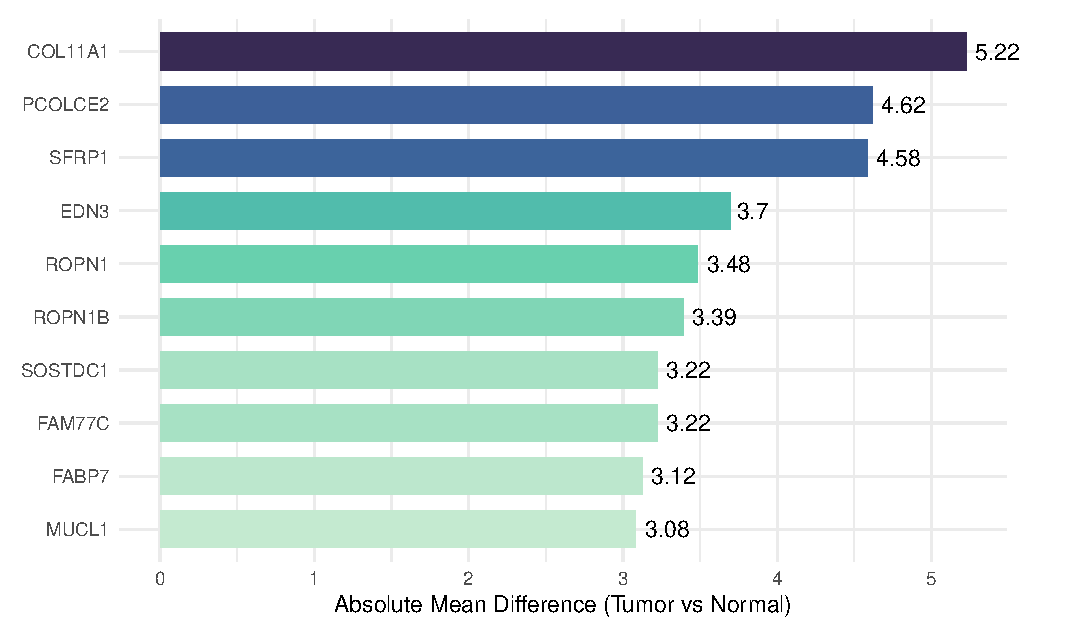
\includegraphics[width=8cm,height=4cm]{Images/AMD.pdf}
		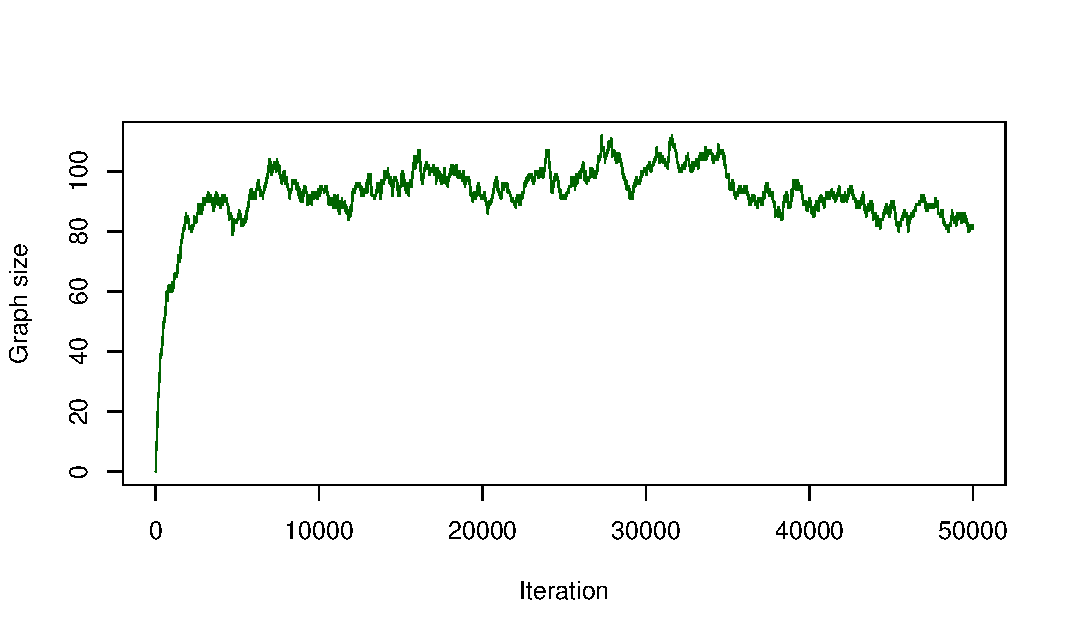
\includegraphics[width=6.5cm,height=5cm]{Images/trace plot of graph size.pdf}
		\vspace{-0.2cm}
		\caption{\footnotesize{TCGA data. Top 10 genes with the highest expression difference between tumor and normal samples. The absolute mean difference in expression levels was calculated for each gene using the TCGA breast cancer dataset. Exact difference values are annotated on the respective bars (left panel). Trace plot of graph size in the DAGs visited by the MCMC at each iteration (right panel).}}\label{fig3}
	\end{center}
\end{figure}
\vspace{-0.6cm}
\begin{figure}[ht]
	\begin{center}
		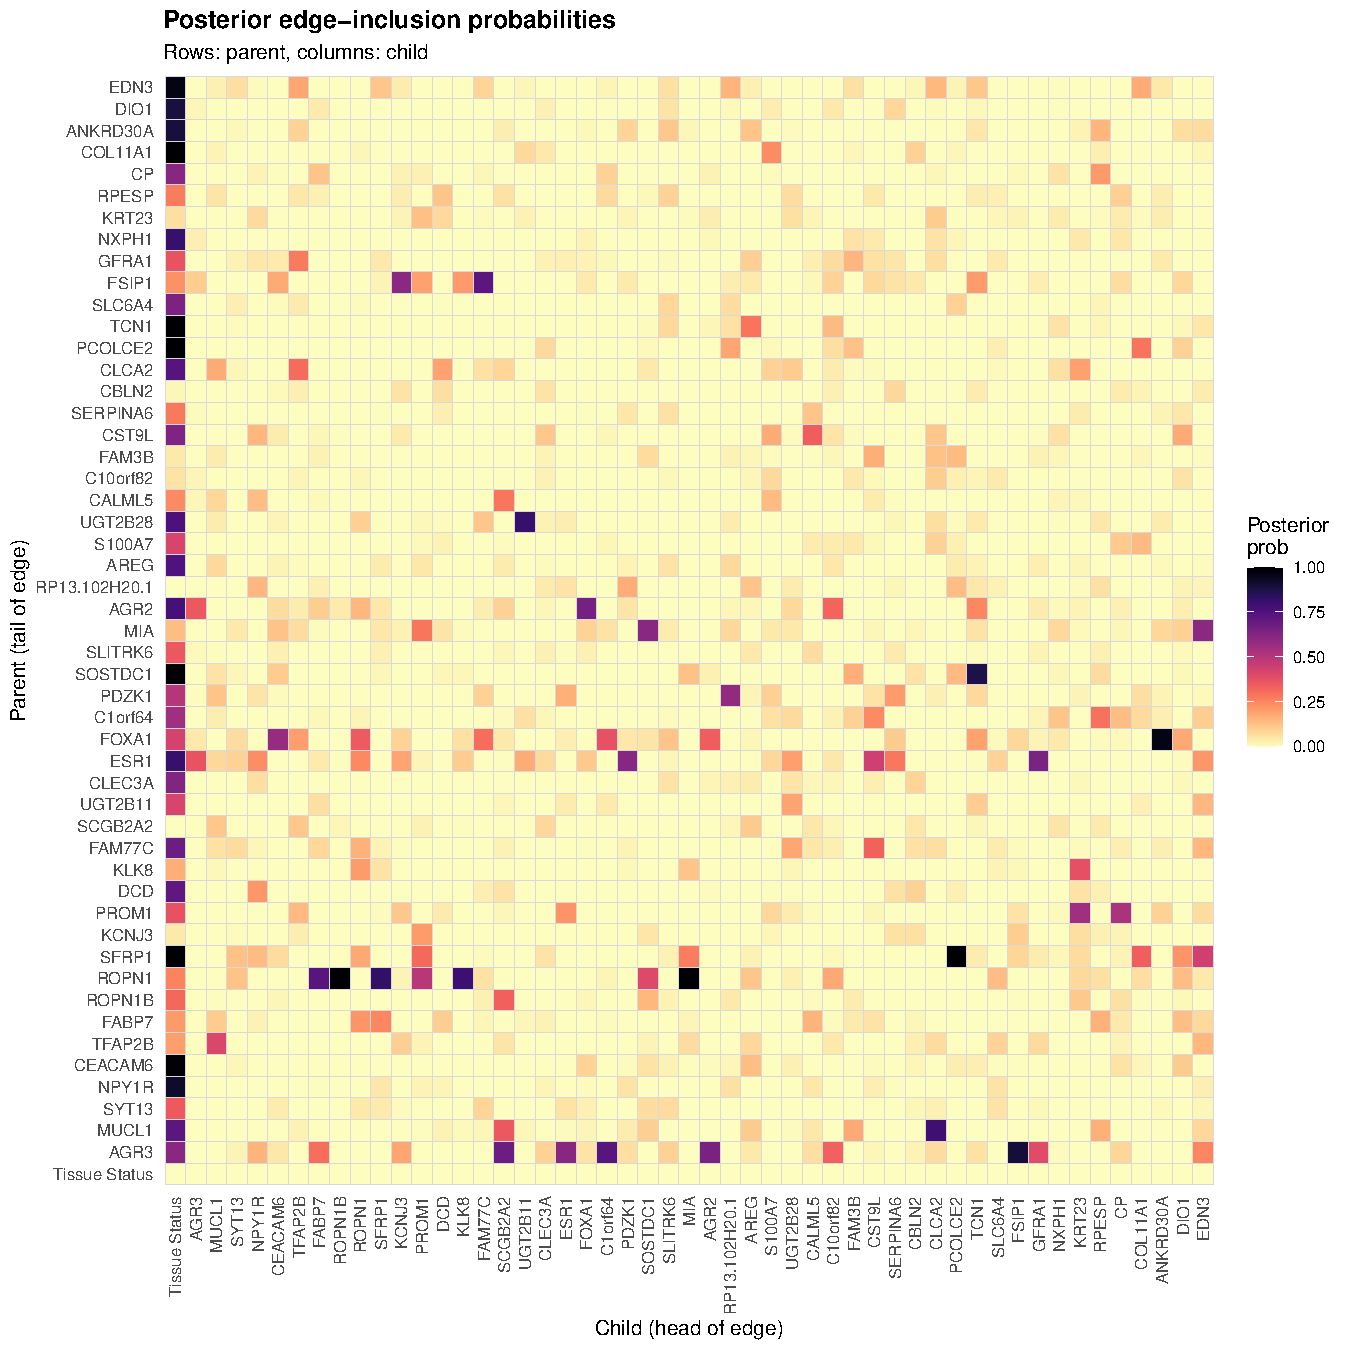
\includegraphics[width=7.2cm,height=4.3cm]{Images/heatmap_real.pdf}
		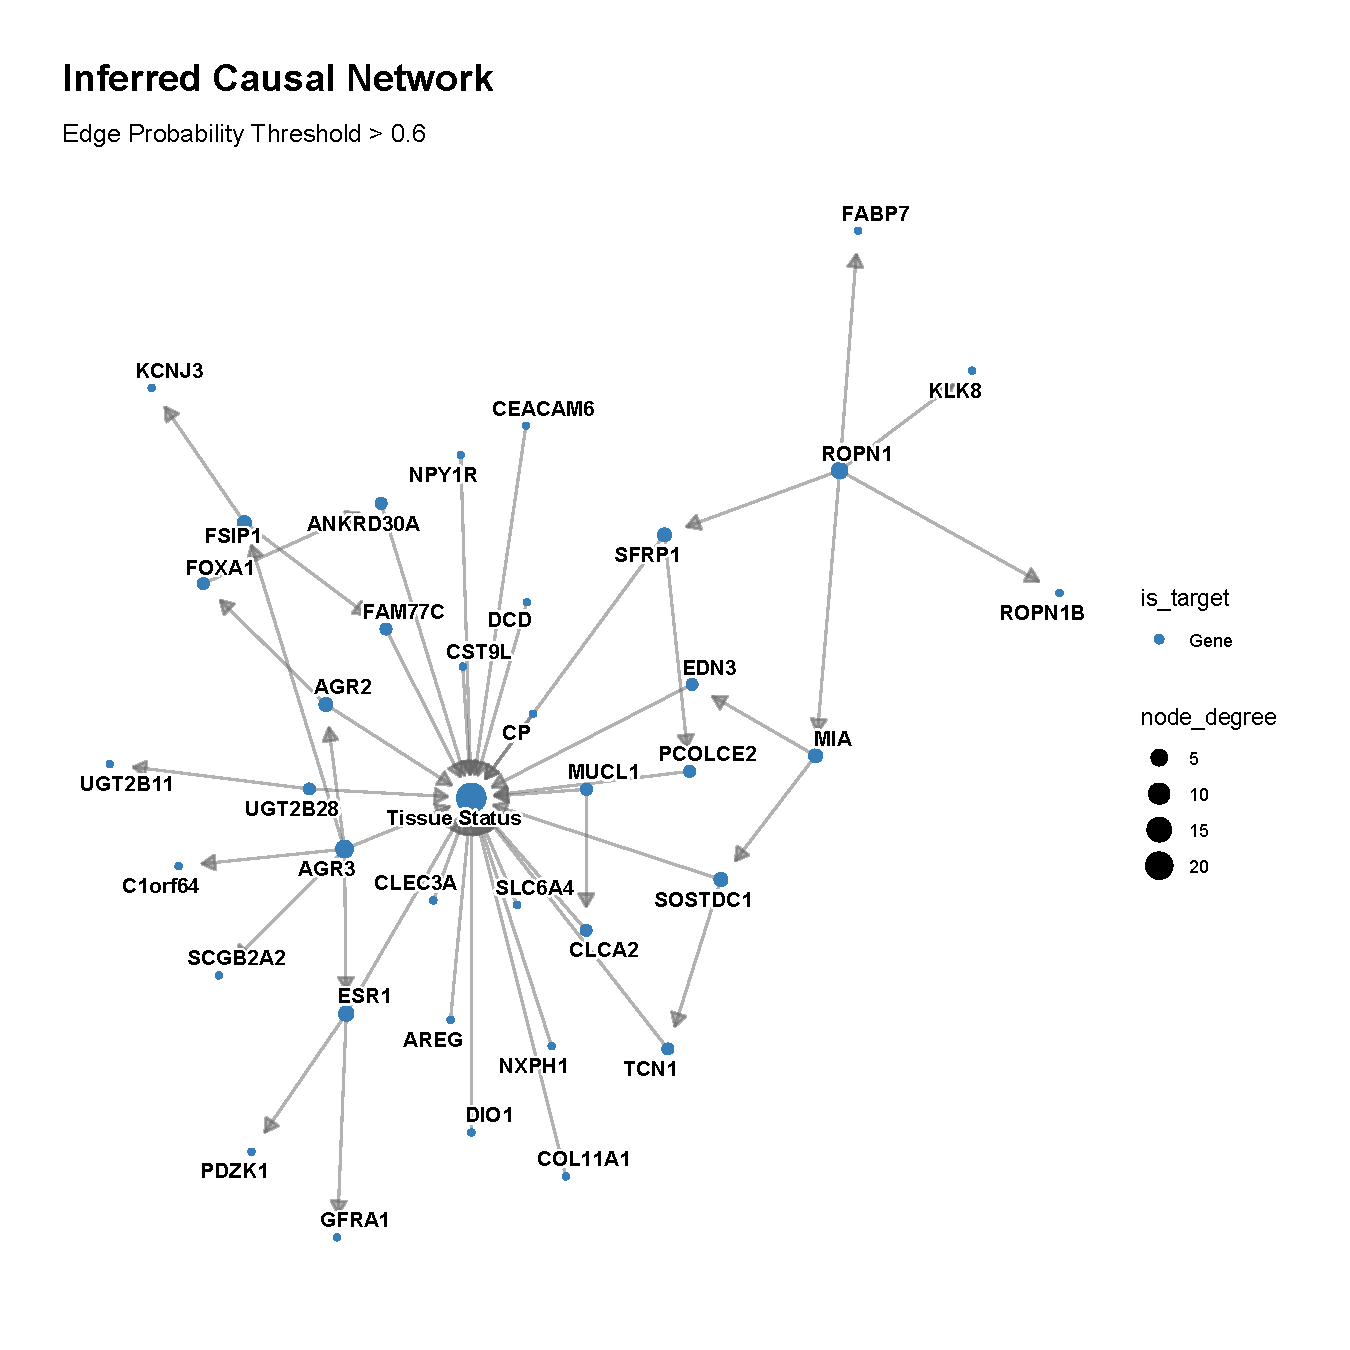
\includegraphics[width=7.2cm,height=4.3cm]{Images/network_real.pdf}\\
		%\vspace{-0.2cm}
		\caption{\footnotesize{TCGA data. Heat map of posterior edge inclusion probabilities across the 50 genes and the tissue status node (left panel). Inferred causal network for breast cancer tissue status. Edges with posterior inclusion probability exceeding 0.6 are shown (right panel).}}\label{fig2}
	\end{center}
\end{figure}

\begin{table}[ht]
	\begin{center}
		\scriptsize
		\caption{Posterior probabilities of inclusion of the directed edge gene $\rightarrow$ tissue status. Top eight entries shown.}\label{tab1}
		\begin{tabular}{|cc|cc|}
			\hline
			Gene & Posterior probability & Gene & Posterior probability \\  \hline \hline
			COL11A1 & 1.00 & SOSTDC1 & 1.00 \\
			PCOLCE2 & 1.00 & CEACAM6 & 0.992  \\
			SFRP1   & 1.00 & EDN3 & 0.965  \\ 
			TCN1   & 1.00 & NPY1R & 0.922 \\ \hline
		\end{tabular}
	\end{center}
\end{table}

\begin{figure}[ht]
	\begin{center}
		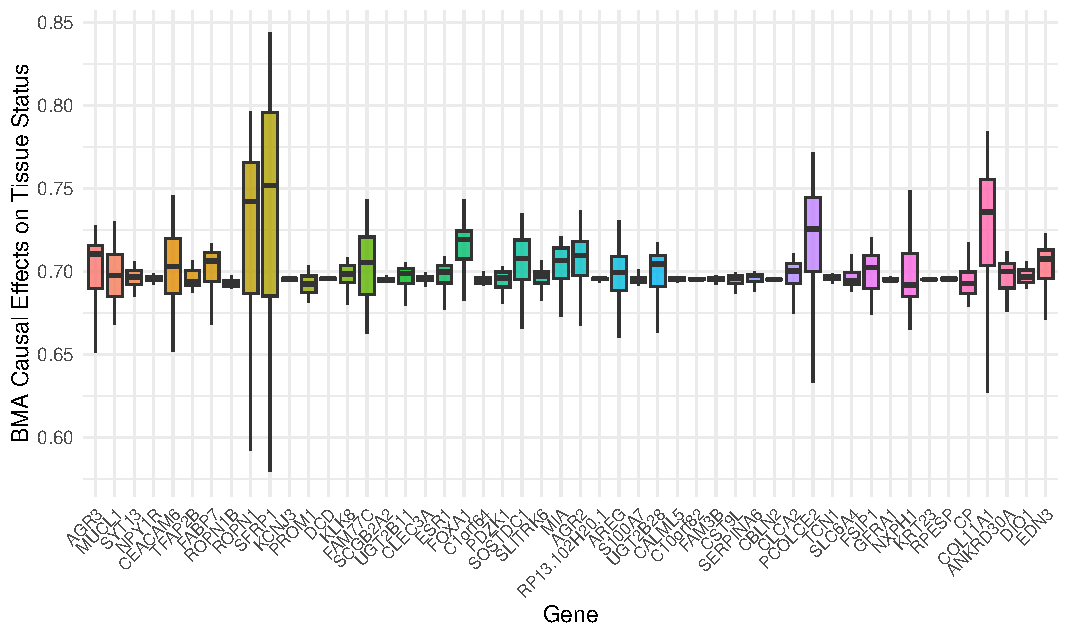
\includegraphics[width=10cm,height=3.5cm]{Images/boxplot_real.pdf}
		\vspace{-0.2cm}
		\caption{\footnotesize{Posterior distribution of BMA causal effects estimates on tissue status.}}\label{fig4}
	\end{center}
\end{figure}
%%%%%%%%%%%%%%%%%%%%%%%%%%%%%%%%%%%%%%%%%%%%%%%%%%%%%%%%%%%%%%%
\vspace{-1.35cm}
\section*{Discussion and Conclusion}
  
%In this paper, our primary objective was to demonstrate the practical applicability of a Bayesian structure learning framework, based on the DAG-probit model and Laplace-approximated scoring, in the context of real-world oncological data. By applying this methodology to the TCGA breast cancer dataset, we successfully inferred a cohesive gene regulatory network that directly links continuous transcriptomic profiles with discrete clinical tissue states.
%
%The application yielded highly interpretable and biologically significant insights into the molecular mechanisms of breast cancer. Most notably, the network effectively isolated the Markov Blanket of the clinical outcome, identifying a robust subset of key biomarkers—\textit{COL11A1}, \textit{PCOLCE2}, \textit{SFRP1}, \textit{TCN1}, and \textit{SOSTDC1}—with a definitive posterior inclusion probability of $1.00$. In addition to identifying direct effects, the model captured deeper hierarchical dependencies, extracting specific directed pathways such as $\textit{ROPN1} \rightarrow \textit{SFRP1} \rightarrow \textit{PCOLCE2} \rightarrow \textit{Tissue Status}$. The strong alignment of these extracted pathways with existing oncology literature underscores the practical value of this approach for targeted biomarker discovery and causal mechanism extraction.
%
%Overall, this empirical study confirms that the methodology discussed by \citep{Nazari:2026} provides a highly effective and reliable analytical pipeline for applied bioinformatics. By translating complex, mixed-type genomic data into actionable biological targets through Bayesian model averaging, it offers substantial utility for clinical research. Future applied studies could leverage this pipeline to analyze other cancer subtypes, integrate diverse multi-omics datasets, or evaluate the prognostic impact of these networks by incorporating patient survival data.
In this paper, we demonstrated the empirical utility of the Bayesian DAG-probit framework \citep{Nazari:2026} by applying it to TCGA breast cancer data. 
By integrating continuous transcriptomic profiles with discrete clinical states, the model inferred a biologically meaningful regulatory network. 
In particular, it identified key biomarkers directly associated with clinical outcome (\textit{COL11A1}, \textit{PCOLCE2}, \textit{SFRP1}, \textit{TCN1}, and \textit{SOSTDC1}) with definitive posterior inclusion probabilities ($1.00$). 
The framework also captured deep hierarchical dependencies, extracting specific directed pathways such as $\textit{ROPN1} \rightarrow \textit{SFRP1} \rightarrow \textit{PCOLCE2} \rightarrow \textit{Tissue Status}$. 
The strong alignment of these findings with existing oncology literature underscores the value of the pipeline for the discovery of targeted biomarkers and the extraction of causal mechanisms from mixed-type data. Future research could extend this approach to multi-omics integration and patient survival analysis across other cancer subtypes.

%\section*{Acknowledgments}   
%If you wish to include acknowledgments, this section should appear before the references.
%%%%%%%%%%%%%%%%%%%%%%%% References %%%%%%%%%%%%%%%%%%%%%%%%%%%%%
\vspace{-0.5cm}\small
\begin{thebibliography}{9}
\bibitem[Castelletti and Consonni (2021)]{Castelletti21}
Castelletti F., Consonni G. (2021), Bayesian causal inference in probit graphical models, {\it Bayesian Analysis}, 16(4), 1113--1137.

\bibitem[Friedman et al. (2000)]{Friedman00}
Friedman N., Linial M., Nachman I., Pe'er D. (2000), Using Bayesian networks to analyze expression data, {\it Proceedings of the fourth annual international conference on Computational molecular biology}, 127--135.

\bibitem[Nazari et al. (2026)]{Nazari:2026}
Nazari S., Arashi M., and Sadeghkhani A. (2026), Scalable Bayesian Structure Learning of Directed Acyclic Graphs via Laplace Approximation, with an Application to Breast Cancer Gene Expression Networks, {\it Submitted for publication}.

\bibitem[Poola et al. (2005)]{Poola05}
Poola I., DeWitty R. L., Marshalleck J. J., Bhatnagar R., Abraham J. and Leffall L. D. (2005), Identification of MMP-1 as a putative breast cancer predictive marker by global gene expression analysis, {\it Nature medicine}, 11(5), 481-483.

\bibitem[Veeck et al. (2006)]{Veeck06}
Veeck J., Niederacher D., An H., Klopocki E., Wiesmann F., Betz B. et al. (2006), Aberrant methylation of the Wnt antagonist SFRP1 in breast cancer is associated with unfavourable prognosis, {\it Oncogene}, 25(24), 3479-3488.

\bibitem[Wang and Wang (2025)]{WW25}
Wang Y. and Wang J. (2025), The Dynamic Changes of COL11A1 Expression During the Carcinogenesis and Development of Breast Cancer and as a Candidate Diagnostic and Prognostic Marker, {\it The breast journal}, 2025(1), 7861864.

\bibitem[Cancer Genome Atlas Network (2012)]{CGAN12}
Cancer Genome Atlas Network (2012), Comprehensive molecular portraits of human breast tumors, {\it Nature}, 490(7418), 61.

\end{thebibliography}
 \end{document}

